% remove "answers" to suppress solutions
\documentclass[11pt,addpoints,answers]{exam}

\usepackage{fullpage}
\usepackage{amsfonts, amsmath, amssymb, amsthm}
\usepackage{mathtools}
\usepackage{enumerate}
\usepackage{listings}
\usepackage[boxed]{algorithm}
\usepackage[noend]{algpseudocode}

\usepackage{hyperref}
\usepackage{tikz}
\usepackage[inline,shortlabels]{enumitem}
\usepackage{subcaption}

% in order to compile this file you need to get 'header.tex' from
% Canvas and change the line below to the appropriate file path
%%% theorems

\theoremstyle{plain}            % following are "theorem" style
\newtheorem{theorem}{Theorem}[section]
\newtheorem{lemma}[theorem]{Lemma}
\newtheorem{corollary}[theorem]{Corollary}
\newtheorem{proposition}[theorem]{Proposition}
\newtheorem{claim}[theorem]{Claim}
\newtheorem{fact}[theorem]{Fact}
\newtheorem{openproblem}[theorem]{Open Problem}

\theoremstyle{definition}       % following are def style
\newtheorem{definition}[theorem]{Definition}
\newtheorem{conjecture}[theorem]{Conjecture}
\newtheorem{example}[theorem]{Example}
\newtheorem{protocol}[theorem]{Protocol}
\newtheorem{exercise}[theorem]{Exercise}

\theoremstyle{remark}           % following are remark style
\newtheorem{remark}[theorem]{Remark}
\newtheorem{note}[theorem]{Note}
\newtheorem*{aside}{Aside}
\newtheorem*{gn}{Grading Note} % grading note

%%% special sets
\newcommand{\bit}{\ensuremath{\{0,1\}}}
\newcommand{\bitt}{\ensuremath{\{-1,1\}}}

% font for general-purpose algorithms
\newcommand{\algo}[1]{\ensuremath{\mathsf{#1}}}
% font for general-purpose computational problems
\newcommand{\problem}[1]{\ensuremath{\mathsf{#1}}}
% font for complexity classes
%\newcommand{\class}[1]{\ensuremath{\mathsf{#1}}}

\global\long\def\path{\mathrm{path}}
% asymptotics
%\DeclareMathOperator{\poly}{poly}
%\DeclareMathOperator{\polylog}{polylog}
\DeclareMathOperator{\negl}{negl}
\DeclareMathOperator{\Otil}{\tilde{O}}
\DeclareMathOperator{\Ostar}{O^*}

%%% "LEFT-RIGHT" PAIRS OF SYMBOLS

% inner product
\DeclarePairedDelimiter\inner{\langle}{\rangle}
% absolute value
\DeclarePairedDelimiter\abs{\lvert}{\rvert}
% a set
\DeclarePairedDelimiter\set{\{}{\}}
% parens
\DeclarePairedDelimiter\parens{(}{)}
% tuple, alias for parens
\DeclarePairedDelimiter\tuple{(}{)}
% square brackets
\DeclarePairedDelimiter\bracks{[}{]}
% rounding off
\DeclarePairedDelimiter\round{\lfloor}{\rceil}
% floor function
\DeclarePairedDelimiter\floor{\lfloor}{\rfloor}
% ceiling function
\DeclarePairedDelimiter\ceil{\lceil}{\rceil}
% length of some vector, element
\DeclarePairedDelimiter\length{\lVert}{\rVert}
% norm
\DeclarePairedDelimiter\norm{\lVert}{\rVert}
% length (as a string)
\DeclarePairedDelimiter\len{\lvert}{\rvert}
% bra-kets
\DeclarePairedDelimiter\bra{\langle}{\rvert}
\DeclarePairedDelimiter\ket{\lvert}{\rangle}
\newcommand{\braket}[2]{\ensuremath{\langle #1 \vert #2 \rangle}}
\newcommand{\ketbra}[2]{\ensuremath{\lvert #1 \rangle \langle #2 \rvert}}

%%% MATH OPERATORS
\DeclareMathOperator{\Var}{Var}
\DeclareMathOperator{\tr}{Tr}
\DeclareMathOperator{\supp}{supp}
\DeclareMathOperator{\var}{var}
\DeclareMathOperator{\vol}{vol}
\DeclareMathOperator{\sign}{sign}

%%% BLACKBOARD SYMBOLS

\newcommand{\C}{\ensuremath{\mathbb{C}}}
\newcommand{\D}{\ensuremath{\mathbb{D}}}
\newcommand{\F}{\ensuremath{\mathbb{F}}}
\newcommand{\G}{\ensuremath{\mathbb{G}}}
\newcommand{\J}{\ensuremath{\mathbb{J}}}
\newcommand{\N}{\ensuremath{\mathbb{N}}}
\newcommand{\Q}{\ensuremath{\mathbb{Q}}}
\newcommand{\R}{\ensuremath{\mathbb{R}}}
\newcommand{\T}{\ensuremath{\mathbb{T}}}
\newcommand{\Z}{\ensuremath{\mathbb{Z}}}
\newcommand{\QR}{\ensuremath{\mathbb{QR}}}

% sets in calligraphic type

\newcommand{\calD}{\ensuremath{\mathcal{D}}}
\newcommand{\calF}{\ensuremath{\mathcal{F}}}
\newcommand{\calG}{\ensuremath{\mathcal{G}}}
\newcommand{\calH}{\ensuremath{\mathcal{H}}}
\newcommand{\calI}{\ensuremath{\mathcal{I}}}
\newcommand{\calL}{\ensuremath{\mathcal{L}}}
\newcommand{\calN}{\ensuremath{\mathcal{N}}}
\newcommand{\calP}{\ensuremath{\mathcal{P}}}
\newcommand{\calS}{\ensuremath{\mathcal{S}}}
\newcommand{\calX}{\ensuremath{\mathcal{X}}}
\newcommand{\calY}{\ensuremath{\mathcal{Y}}}

% matrices and vectors

\newcommand{\matA}{\ensuremath{\mathbf{A}}}
\newcommand{\matB}{\ensuremath{\mathbf{B}}}
\newcommand{\matC}{\ensuremath{\mathbf{C}}}
\newcommand{\matD}{\ensuremath{\mathbf{D}}}
\newcommand{\matE}{\ensuremath{\mathbf{E}}}
\newcommand{\matF}{\ensuremath{\mathbf{F}}}
\newcommand{\matG}{\ensuremath{\mathbf{G}}}
\newcommand{\matH}{\ensuremath{\mathbf{H}}}
\newcommand{\matI}{\ensuremath{\mathbf{I}}}
\newcommand{\matJ}{\ensuremath{\mathbf{J}}}
\newcommand{\matK}{\ensuremath{\mathbf{K}}}
\newcommand{\matL}{\ensuremath{\mathbf{L}}}
\newcommand{\matM}{\ensuremath{\mathbf{M}}}
\newcommand{\matN}{\ensuremath{\mathbf{N}}}
\newcommand{\matO}{\ensuremath{\mathbf{O}}}
\newcommand{\matP}{\ensuremath{\mathbf{P}}}
\newcommand{\matQ}{\ensuremath{\mathbf{Q}}}
\newcommand{\matR}{\ensuremath{\mathbf{R}}}
\newcommand{\matS}{\ensuremath{\mathbf{S}}}
\newcommand{\matT}{\ensuremath{\mathbf{T}}}
\newcommand{\matU}{\ensuremath{\mathbf{U}}}
\newcommand{\matV}{\ensuremath{\mathbf{V}}}
\newcommand{\matW}{\ensuremath{\mathbf{W}}}
\newcommand{\matX}{\ensuremath{\mathbf{X}}}
\newcommand{\matY}{\ensuremath{\mathbf{Y}}}
\newcommand{\matZ}{\ensuremath{\mathbf{Z}}}
\newcommand{\matzero}{\ensuremath{\mathbf{0}}}

\newcommand{\veca}{\ensuremath{\mathbf{a}}}
\newcommand{\vecb}{\ensuremath{\mathbf{b}}}
\newcommand{\vecc}{\ensuremath{\mathbf{c}}}
\newcommand{\vecd}{\ensuremath{\mathbf{d}}}
\newcommand{\vece}{\ensuremath{\mathbf{e}}}
\newcommand{\vecf}{\ensuremath{\mathbf{f}}}
\newcommand{\vecg}{\ensuremath{\mathbf{g}}}
\newcommand{\vech}{\ensuremath{\mathbf{h}}}
\newcommand{\veck}{\ensuremath{\mathbf{k}}}
\newcommand{\vecm}{\ensuremath{\mathbf{m}}}
\newcommand{\vecp}{\ensuremath{\mathbf{p}}}
\newcommand{\vecq}{\ensuremath{\mathbf{q}}}
\newcommand{\vecr}{\ensuremath{\mathbf{r}}}
\newcommand{\vecs}{\ensuremath{\mathbf{s}}}
\newcommand{\vect}{\ensuremath{\mathbf{t}}}
\newcommand{\vecu}{\ensuremath{\mathbf{u}}}
\newcommand{\vecv}{\ensuremath{\mathbf{v}}}
\newcommand{\vecw}{\ensuremath{\mathbf{w}}}
\newcommand{\vecx}{\ensuremath{\mathbf{x}}}
\newcommand{\vecy}{\ensuremath{\mathbf{y}}}
\newcommand{\vecz}{\ensuremath{\mathbf{z}}}
\newcommand{\veczero}{\ensuremath{\mathbf{0}}}
\newcommand{\vecone}{\ensuremath{\mathbf{1}}}

%%% misc

\newcommand{\eps}{\varepsilon}

%%% for homework and section notes

\newcommand{\commonheader}[2]{
    \pagestyle{headandfoot}
    \setlength{\headheight}{26pt}
    \setlength{\headsep}{16pt}

    \header
        {\small{\textbf{EECS 376: Foundations of Computer Science}} \\ \footnotesize{\textbf{University of Michigan, Spring 2024}}}
        {#1}
        {#2}

    \firstpageheadrule
    \runningheadrule

    \footer
        {}
        {\thepage}
        {}
}

\newcommand{\hwheader}{
    \commonheader
        {\Large \textbf{Homework \hwnum}}
        {\small \textbf{Due 8:00pm, \duedate\\ {\tiny(accepted until 9:59 pm, no credit after)}}}
}

\newcommand{\hwslnheader}{
    \commonheader
    	{}
        {\Large \textbf{Solutions to Homework \hwnum}}
    \printanswers
}

\newcommand{\notesheader}{
    \commonheader
    	{}
        {\Large \textbf{Discussion Notes \sectionnum}}
}

\newcommand{\practiceheader}{
    \commonheader
    	{}
        {\Large \textbf{Discussion Worksheet \sectionnum}}
}

\newcommand{\practiceslnheader}{
    \commonheader
    	{}
        {\Large \textbf{Solutions to Discussion Worksheet \sectionnum}}
}

\newcommand{\reviewheader}{
    \commonheader 
    \smallskip
    	{}
        {\Large \textbf{Midterm Review Notes}}
}

\newcommand{\hwpreface}{

\noindent This homework has \numquestions\ questions, for a total of \numpoints\ points and \numbonuspoints\ extra-credit points.

\noindent Unless otherwise stated, each question requires \emph{clear}, \emph{logically correct}, and \emph{sufficient} justification to convince the reader.

\noindent For bonus/extra-credit questions, we will provide very limited guidance in office hours and on Piazza, and we do not guarantee anything about the difficulty of these questions.
 
\noindent We strongly encourage you to typeset your solutions in \LaTeX.

\noindent If you collaborated with someone, you must state their name(s). You must \emph{write your own solution} for all problems and \emph{may not use any other student’s write-up}.
}

\newcommand{\hint}[1]{
\emph{Hint}: #1
}
\newcommand{\bonus}{
\emph{Optional bonus}:
}
\newcommand{\extracredit}{
\emph{Extra credit}: 
}


\algnewcommand{\algorithmiconinput}[2]{\text{#1 = ``on input #2:}}

% P, NP, NP-Hard, NP-Complete, poly-reduction
\newcommand{\NP}{\textsf{NP}}
\renewcommand{\P}{\textsf{P}}
\newcommand{\NPHard}{\NP\text{-Hard}}
\newcommand{\NPComplete}{\NP\text{-Complete}}
\newcommand{\ptimemap}{\leq_p}

% Languages in this HW
\newcommand{\atm}{L_{\text{ACC}}}
\newcommand{\htm}{L_{\text{HALT}}}
\newcommand{\SAT}{\text{SAT}}
\newcommand{\HamTrek}{\textsc{Ham-Trek}}
\newcommand{\HamPath}{\textsc{Ham-Path}}
\newcommand{\Knapsack}{\textsc{Knapsack}}
\newcommand{\SubsetSum}{\textsc{SubsetSum}}
\newcommand{\clique}{\textsc{Clique}}
\renewcommand{\triangle}{\textsc{Triangle}}
\newcommand{\halfclique}{\textsc{Half-Clique}}

\newcommand{\hwnum}{4}
\newcommand{\duedate}{June 13}
\usepackage{xcolor}

\hwheader  

% Comment the following line in order to hide solutions.
% Uncomment the line to show solutions written inside of
% LaTeX solution environments like:
%   \begin{solution}
%     My solution.
%   \end{solution}.

\begin{document}

\hwpreface

\pointsinmargin
\pointpoints{pt}{pts}
\bonuspointpoints{EC pt}{EC pts}
\marginpointname{ \points}
\marginbonuspointname{ \bonuspoints}

\begin{questions}
  \addtocounter{question}{-1}

  \question[0] \textbf{Before you start; before you submit.}

  \begin{parts}
      \part Carefully read \href{https://drive.google.com/file/d/1Nk6EPiQZlplO856LTpcMbw7xY7QdHxia/view?usp=drive_link}{Handout 3} before starting this assignment, and apply it to the solutions you submit.
      \part If applicable, state the name(s) and uniqname(s) of your collaborator(s).
  \end{parts}
  
  \begin{solution}
None.
  \end{solution}
  
  \question[10] \textbf{Self assessment.}
  
  Carefully read and understand the posted solutions to the \textbf{midterm exam}.
  Identify \textbf{one long-answer question} for which your own solution has the most room for improvement (e.g., has unsound reasoning, doesn’t show what was required, could be significantly clearer or better organized, etc.).
  Copy or screenshot this solution, then in a few sentences, explain what was deficient and how it could be fixed.

  (Alternatively, if you think one of your solutions is significantly \emph{better} than the posted one, copy it here and explain why you think it is better.)

  You may reference the answer key, but your answer should be in your own words.

  \begin{solution}
    \begin{center}
      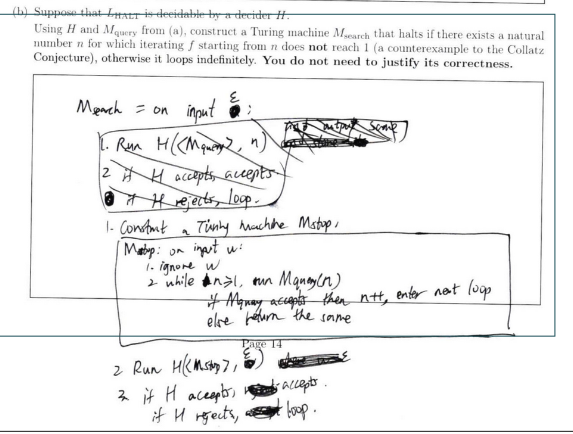
\includegraphics[scale=0.7]{1.png}\\
    \end{center}
    I did not work out the first long answer since I cannot think of the greediness inside the dp, so I think maybe I cannot improve that during exam. But I did work out the second long answer, while I did not get point for the (b) part, so I think I should have made it right if I were more careful. I makes this question more complex than it should be which is also wrong answer, since I did not consider carefully that if $M_{query}$ did not halt on a natural number $n$, then it will loop infinitely, causing the $H$ to reject, which cause the result to loop. Therefore in both way, the $M_{stop}$ will loop and the $H$ will reject, so the $M_{search}$ will not halt on any input. Acctualy I do not need to construct any extra Turing Machine. It is fine to just iterate on natural number $n$ and run $H(<M_{query}>, n)$ for each $n$.
  \end{solution}

    \question \textbf{\P\ \NP\ MAMC.} 

    For each of the following multiple-answer multiple choice question, select all correct options. While justification is \textbf{not required} to received for full credit, providing it is highly encouraged. \textit{Note: If you are editing the \LaTeX \ file, change} \texttt{choice} \textit{to} \texttt{CorrectChoice} \textit{to fill in the bubble.}
    
    \begin{parts}
        \part [5] Let $A$ and $B$ be two languages. Suppose $A \ptimemap B$, which of the following statement(s) is/are necessarily true? 
        
        \begin{checkboxes}
            \choice If $A$ is in $\P$ then $B$ is in $\P$.
            \choice If $A$ is in $\P$, then $B$ is in $\NP$.
            \CorrectChoice If $A$ is $\NPHard$, then $B$ is $\NPHard$.
            \CorrectChoice If $A$ is $\NPComplete$, then $B$ is $\NPHard$.
            \choice Both $A$ and $B$ are in $\P$ or neither $A$ nor $B$ is in $\P$.
        \end{checkboxes}
        \begin{solution}

        \end{solution}

        \part [5] Which of the following statements, if true, would imply $\P = \NP$?  
        \begin{checkboxes}
            \choice There exists a language in $\NP$ but that is not in $\P$.
            \choice Some NP language $L$ is in $\P$.
            \CorrectChoice $\SAT$ can be solved in $O(n^6)$ time.
            \choice There exists an $\NPComplete$ language that is $\NPHard$.
            \CorrectChoice  $L_{\text{even}}= \set{n : n \text{ is even}}$ is NP-complete.
        \end{checkboxes}

        \begin{solution}

        \end{solution}

        \part [5] Suppose $\P \neq \NP$, which of the following statement(s) is/are true?

        \begin{checkboxes}
            \CorrectChoice $\NPComplete$ languages cannot be decided efficiently.
            \CorrectChoice If $L$ is $\NPHard$, then $L \not\in \P$.
            \choice If $\overline{L}$ is $\NPHard$, then $L$ is not in $\P$.
            \choice Every language in the class $\NP$ is also $\NPHard$.
            \CorrectChoice $L_\text{odd} = \set{n : n \text{ is odd}}$ is not $\NPComplete$.
        \end{checkboxes}
        \begin{solution}

        \end{solution}
    \end{parts}

  \question \textbf{Understanding $\P$, $\NP$, and poly-time mapping reductions.}
  
  \begin{parts}
        
    \part[5] We claim that $\P \subseteq \NP$, i.e., for any language $L \in \P$, we have that $L \in \NP$ as well.
    Here is an \emph{incomplete} proof of this fact, which you will complete.
    
    By the hypothesis that $L \in \P$, there is an efficient Turing machine~$M$ that decides~$L$.
    We define the following efficient verifier~$V$ for~$L$.
    
    \begin{algorithmic}[1]
      \Function{$V$}{$x,c$}
      \State \textbf{[MISSING PSEUDOCODE]}
      \EndFunction
    \end{algorithmic}
    
    State what the missing pseudocode should be, and prove that~$V$ is indeed an efficient verifier for~$L$.

    \begin{solution}

    \begin{algorithmic}[1]
        \Function{$V$}{$x,c$}
        \State Ignore $c$
        \State Run $M$ on input $x$
        \If{$M$ accepts $x$}
            \State \Return TRUE
        \Else
            \State \Return FALSE
        \EndIf
        \EndFunction
    \end{algorithmic}
    V is an efficient verifier for $L$ because if $x\in L$, then $M$ accepts $x$ and so take some arbitrary dummit $c$ we have $V(x,c)$ accepts $x$; if $x \not\in L$ then $M$ rejects $x$, so for all $c$ we have $V(x,c)$ rejects $x$; And $V(x,c)$ runs in polynomial time since $M$ runs in polynomial time.
    \end{solution}   

    \part[8] Show that poly-time mapping reductions are transitive.
    That is, if $A \ptimemap B$ and $B \ptimemap C$, then $A \ptimemap C$.

    \begin{solution}
    Assume the hypothesis. Then there exists some function $f: \Sigma^{*} \rightarrow \Sigma^{*}$ such that for all $x \in \Sigma^{*}$, if $x \in A$ then $f(x) \in B$ and if $x \not\in A$ then $f(x) \not\in B$.
    \\And there exists some function $g: \Sigma^{*} \rightarrow \Sigma^{*}$ such that for all $y \in \Sigma^{*}$, if $y \in B$ then $g(y) \in C$ and if $y \not\in B$ then $g(y) \not\in C$.
    
    So now we consider the function $f \circ g$.\\
    Let $x\in A$ be arbitrary, then $f(x) \in B$, so $g \circ f(x) = g(f(x)) \in C$.\\
    Let $x \not\in A$ be arbitrary, then $f(x) \not\in B$, so $g \circ f(x) = g(f(x)) \not\in C$.
    \\This finishes the proof.
    \end{solution}

    \part[8] Let $C = A \cup B$ where both $A, B$ are languages in $\NP$.
    State, with proof, whether~$C$ is in $\NP$ for \emph{all}, \emph{some} (but not all), or \emph{no} such $A,B$.
         
    \begin{solution}
  Claim: $C = A \cup B$ is in $\NP$, for all such $A,B$.
\\Proof:
\\Consider the following verifier for $C$:\\
Let $V_A$ be a verifier for $A$ and $V_B$ be a verifier for $B$.\\
\textbf{Input}: $x \in A \cup B$, $c = (i, c')$ where $i \in {0,1}$ and $c'$ is a certificate for either $V_A$ or $V_B$. 
\begin{algorithmic}[1]
        \Function{$V$}{$x,c$}
        \If{$i = 0$}
            run $V_A(x, c')$
        \Else{}
            run $V_B(x, c')$
        \EndIf
        \EndFunction
    \end{algorithmic}
    if $x \in A \cup B$, then $x \in A$ or $x \in B$, so if $x \in A$ then there exists some $c'$ such that $(0,c')$ verifies $x$ in polynomial time, and if $x\in B$ then there exists some $c'$ such that $(1,c')$ verifies $x$ in polynomial time, since $V_A$ and $V_B$ run in polynomial time. If $x \not\in C$, then $x \not\in A$ and $x \not\in B$, so for all $c$ we have $V(x,c)$ rejects $x$.
    \end{solution}
  \end{parts}

   \question \textbf{SAT Review.}
    \begin{parts}
    \part[5] Briefly explain what the ``Boolean satisfiability'' ($\SAT$) problem is, and give one example instance that is satisfiable, and one that is unsatisfiable.
    Each example must include at least 2 variables and at least 3 (not necessarily distinct) logical operators (AND/OR/NOT).
    
    \begin{solution}
    ``SAT" problem: Given a Boolean formula(which is made up of literals, ORs and ANDs, where literals means variables and their negations), output whether there is an assignment of truth values to the variables that makes the formula true.\\

    Example of satisfiable instance: $(x_1 \vee x_2) \wedge (\neg x_1 \vee x_2) \wedge (x_1 \vee \neg x_2)$, where $x_1 = T, x_2 = F$\\
    Example of unsatisfiable instance: $(x_1 \vee x_2) \wedge (\neg x_1 \vee x_2) \wedge (x_1 \vee \neg x_2) \wedge (\neg x_1 \vee \neg x_2)$ since whatever truth value we give to $x_1$ and $x_2$, there is always a false clause, so the formula is always false.
    \end{solution}
    
    \part[5] Towards proving the Cook-Levin Theorem in lecture, we outlined a proof of the following statement: 
    \begin{quote}
      Let language $L \in \NP$ be arbitrary, and fix an efficient verifier $\textsc{VerifyL}$ for~$L$.
      Given any instance $x$ of $L$, in polynomial time we can construct an instance $\phi$ of $\SAT$ such that $\phi$ is satisfiable \emph{if and only if} there \emph{exists} a $c$ such that the tableau of $\textsc{VerifyL}(x,c)$ has $q_\text{accept}$ in it.
    \end{quote}
    Briefly explain why proving this statement proves that SAT is $\NPHard$.
    
    \begin{solution}
    By proving this statement, we show that for any language $L$ in $\NP$, there exists some mapping $f$ that maps every instace $x$ of $L$ to an instance $\phi$ in $SAT$, and $f(x) \in SAT$ iff $x\in L$, which by definition means that for arbitrary $L\in NP$, $L \ptimemap SAT$, which by definition means that SAT is $\NPHard$.
    \end{solution}
  \end{parts}

    \question \textbf{The Greak Ham Trek.}
    
    As a student at the University of Michigan, you're planning ``The Great Ham Trek," a challenge to navigate from Burton Memorial Tower to the Michigan Union. The goal is to visit exactly $k$ campus buildings, hosting mini-symposia on topics from ham radio innovation to the linguistics of ducks, without retracing your steps.

    Formally, we define the following language:
    \[
        \HamTrek = \left\{
        \begin{aligned}
        (G=(V,E),s,t,S,k) :~ &\text{$G$ has a simple path from $s$ to $t$ that}\\
        &\text{visits \textbf{exactly} $k$ of the vertices in $S$}
        \end{aligned}
        \right\}
    \]
    Note: A \textit{simple path} is a path without a cycle.

    \begin{parts}
        \part [8] Prove that $\HamTrek$ is efficiently verifiable, i.e., $\HamTrek \in \NP$. Specifically, design and analyze (both correctness and runtime) an efficient verifier for $\HamTrek$. 
        \begin{solution}
    Consider the following verifier:\\
    \textbf{Input}:$(G = (V, E), s, t, S, k, p)$ where $G$ is a graph, $s,t in V$, $S\subseteq V$, $k$ is an integer; and a path $p$ in $G$ as certificate.

\begin{algorithmic}[1]
 \Function{$Verify$}{$G, s, t, S, k, p$}
    \If{$k <0$ or $k> |V|$ or}
    \State \Return FALSE
    \EndIf
   \If{$p[0] \neq s $ or $ p[\text{end}] \neq t$}
     \State \Return FALSE
  \EndIf
     \State $visited \gets \text{set()}$
   \State $count \gets 0$
   \For{$i$ from $0$ to $\text{length}(p)-1$}
     \If{$(p[i], p[i-1]) \notin E$}
       \Return FALSE
    \EndIf
    \If{$p[i] \in visited$}
      \Return FALSE
    \Else
     \State $visited$.add($ p[i]$)
    \EndIf
    \If{$p[i] \in S$}
      \State $count \gets count + 1$
    \EndIf
  \EndFor
  \If{$count \neq k$}
    \State \Return FALSE
  \EndIf
  \State \Return TRUE
 \EndFunction
\end{algorithmic}
Now we analyze the correctness and runtime of the verifier.\\
\textbf{Correctness}: If $p$ is a path from $s$ to $t$ that visits exactly $k$ vertices in $S$, then the verifier will return TRUE. 
If $p$ is not a HamTrek, then either $p$ is not a path from $s$ to $t$, or it visits more or less than $k$ vertices in $S$, or it contains a path that does not exists, or it turns back. In all such cases, the verifier will return FALSE.\\
\textbf{Runtime}: The verifier runs in $O(|V|^2)$ time, where $|V|$ is the length of the vertices set, since we iterate in the length of the path which is at most $|V|$, and in each iteration we iterate the visited vertice set which is at most as big as $|V|$ to confirm whether a vertice has been visited. Therefore the verifier is efficient.
        \end{solution}
        
        \part [8] Prove that $\HamTrek$ is $\NPHard$, by showing $\HamPath \ptimemap \HamTrek$, where
        \[
            \HamPath = \set{ (G, s, t) : \text{$G$ is a graph with a Hamiltonian path from $s$ to $t$}}.
        \]
        Note: A Hamiltonian path is a path that visits each vertex of the graph exactly once.

        \begin{solution}
To show $\HamTrek$ is $\NPHard$, we construct a polynomial-time reduction from $\HamPath$ to $\HamTrek$. 
\\My construction: Given an instance $x = (G, s, t)$, map it to an instance for $\HamTrek$ as follows:
Use the same graph $G$, vertice $s$ and $t$.
Set $S = V$, the set of all vertices in $G$.
Set $k = |V|$.
Then the constructed instance is $\phi(x) = (G, s, t, S, k)$.
Now we prove the correctness of the polynomial-time reduction.\\
\textbf{Correctness}:
    If $x = (G, s, t) \in \HamPath$, then by definition, there is a simple path visiting each vertex exactly once, thus visiting exactly $|V|$ vertices between $s$ and $t$, which matches our $k$, so the constructed $\phi(x) = (G,s,t,S,k) \in \HamTrek.$\\\\
    If the constructed instance $\phi(x) = (G, s, t, S, k) \in \HamTrek$, then there exists a simple path from $s$ to $t$ visiting exactly $|V| - 1$ vertices. Given that $S = V$, this path must visit each vertex exactly once, except possibly $s$ or $t$ once more, forming a Hamiltonian path, so $x \in Hampath$.\\\\
    Constructing the $\HamTrek$ instance from a $\HamPath$ instance involves only copying the graph, which is $O(|G|)$, in polynomial time with the input graph $x$.\\

Therefore $Hampath \ptimemap \HamTrek$, and since $HamPath$ is $\NPHard$, we have proved that $\HamTrek$ is $\NPHard$.
        \end{solution}
        
    \end{parts}
    
    \question [8] \textbf{More Knapsack!} 
    
    Recall the $0$-$1$ knapsack problem: an instance is a list of~$n$ item weights $W = (W_1, W_2, \ldots, W_n)$, their corresponding values $V = (V_1, V_2, \ldots, V_n)$, and a weight capacity~$C$. (All values are non-negative integers.) The goal is to select items having maximum total value, such that their total weight does not exceed the capacity.
    
    We can make this a decision problem by introducing a ``budget''~$K$ and asking whether a total value of at least~$K$ can be achieved (again, subject to the capacity constraint):
    
    \[ 
        \Knapsack = \set{ (W, V, C, K) : \exists\; S\subseteq \set{1,\ldots,n} \text{ such that } \sum_{i\in S} W_{i} \leq C \text{ and } \sum_{i\in S} V_{i} \geq K }.
    \]

    Prove that $\Knapsack$ is $\NPHard$, by showing that $\SubsetSum \ptimemap \Knapsack$, where
    
    \[ 
        \SubsetSum = \set{(A, s) : A \text{ is a \emph{multiset} of integers $\geq 0$, and } \exists\; I \subseteq A \text{ such that } \sum_{a \in I} a = s}.
    \]
    
    A \href{https://en.wikipedia.org/wiki/Multiset}{\emph{multiset}}~$A$ is just like a set, but it can have duplicate elements. A submultiset $I \subseteq A$ also can have duplicate elements, as long as it does not have more copies of an particular element than~$A$ does.\footnote{In class we defined a slightly different version of $\SubsetSum$ with ordinary sets instead of multisets. With a little more work, the version with ordinary sets can also be proved $\NPComplete$.}

    \begin{solution}\\
\textbf{Construction}:
\\\textbf{Input}: $(A, s)$ where $A$ is a multiset of integers $\geq 0$ and $s$ is an positive integer.
\\\textbf{Output}:We take $W = V=A, C=K=s$, and take $\phi(A, s) = (W,V,C,K)$ as output.
\\\textbf{Correctness}:\\
If $(A,s) \in \SubsetSum$, then $s = C \leq C$ and $s = K \geq K$, so $\phi(x) \in \Knapsack$. \\
If $\phi(x) \in \Knapsack$, then some of the knapsack items has a total weight of $\leq C = s$ and a total value of $\geq K = s$. Since $W = V$, each item's weight equals its value, so the total weight and total value of these items are both $s$, which implies that there is a submultiset of A that sum up to $s$, so $(A,s) \in \SubsetSum$.
And the construction of $\phi$ is efficient, since it only involves copying the input, which is $O(|A|)$, so $\SubsetSum \leq_p \Knapsack$ as needed. Since $\SubsetSum$ is $\NP$-Hard, we have shown that $\Knapsack$ is $\NP$-Hard.
    \end{solution}

    \question \textbf{More Clique!} 
    
    Recall that a \emph{clique} of an undirected graph $G$ = $(V,E)$ is a subset $C \subseteq V$ such that every pair of vertices in $C$ has an edge between them. A clique with $k$ vertices is refer to as a $k$-clique. In lecture, we proved that $\clique\in\NP$, where
    \[
        \clique = \set{(G = (V,E), k) : G \text{ has a clique of size}\geq k}.
    \]
    
    \begin{parts}
    
    \part [8] A \emph{triangle} in an undirected graph is a 3-clique. Consider the following variant of $\clique$
        \[
            \triangle = \set{G = (V,E): G \text{ has a triangle}.}
        \]
        Show that $\triangle \in \P$.
    
    \begin{solution}
    We construct a decider for $\triangle$ as follows:\\
    \textbf{Input}: $G = (V,E)$ where $G$ is a graph.\\
    \begin{algorithmic}[1]
        \Function{$\triangle$}{$G$}
        \For{each $v \in V$}
            \For{each $u \in V$}
                \If{$(v,u) \in E$}
                    \For{each $w \in V$}
                        \If{$(u,w) \in E$ and $(v,w) \in E$}
                            \State \Return TRUE
                        \EndIf
                    \EndFor
                \EndIf
            \EndFor
        \EndFor
        \State \Return FALSE
        \EndFunction
    \end{algorithmic}
    \textbf{Correctness}: If $G$ has a triangle, then there exists three vertices $v,u,w$ such that $(v,u), (u,w), (v,w) \in E$, so the decider will return TRUE. If $G$ does not have a triangle, then for all $v,u,w$ we have $(v,u), (u,w), (v,w) \not\in E$, so the decider will return FALSE.\\
    \textbf{Runtime}:The decider runs in $O(|V|^3)$ time, since we iterate through all the vertices and for each pair of vertices we check if there is an edge between them, and if there is, we check if there is an edge between the third vertex and the other two vertices. Therefore the decider is efficient.
    \\By the correctness and runtime analysis, we have shown that $\triangle \in \P$.
    \end{solution}
    
    \part [12] Now, consider another  variant of \clique{}:
    \[
        \halfclique = \set{G = (V,E): G \textrm{ has a clique of size}\geq |V|/2.} 
    \]
    
    Prove that $\halfclique$ is \NP-complete.
    
    \begin{solution}\\
\textbf{Claim 1: \(\halfclique \in\) NP}

Consider the following Verifier for \(\halfclique\):\\
Input: \((G = (V, E), p)\) where \(G\) is a graph and $p \subseteq V$ is a set of vertices in $G$.\\
\begin{algorithmic}[1]
    \Function{$Verify$}{$G, p$}
    \If{$|p| < |V|/2$}
        \State \Return FALSE
    \EndIf
    \For{$i = 0$ to $|p|-1$}
        \For{$j = i+1$ to $|p|-1$}
            \If{$(p[i], p[j]) \notin E$}
                \State \Return FALSE
            \EndIf
        \EndFor
    \EndFor
    \State \Return TRUE
    \EndFunction
\end{algorithmic}

\textbf{Correctness}:
The verifier is correct since if $G \in \halfclique$, then there exists a clique of size at least $|V|/2$ in $G$, so by taking vertices in the clique as $p$, the verifier will return TRUE. If $G \not\in \halfclique$, then there is no clique of size at least $|V|/2$ in $G$, so for all $p \subset V$, $Verify(G,p)$ return FALSE.\\
\textbf{Efficiency}:
The verifier runs in polynomial time $O(|V|)^2$ since it iterates through all pairs of vertices in \(p\) for two nested loops, with the size of each at most $|V|$.\\

Above we have proved the correctness and efficiency of the verifier, so \(\halfclique \in \NP\).

\textbf{Claim 2: $\halfclique \in$ NP-Hard}

We show that $\halfclique$ is $\NP-Hard$ by showing that $\clique \ptimemap \halfclique$.\\,

\textbf{Construction}:\\
Input: An instance of \(\clique\) \(x =(G,k)\) specified by a graph \(G = (V, E)\) and an integer \(k\).
\\Output: A graph \(\phi(x) = (V',E')\) as follows:

If \(k \geq {|V|\over 2}\), then initialize $V' = V$ and add $2k - |V|$ vertices to $V'$, so $|V'| = 2k$. Set $E' = E$, and return \(\phi(x) = (V', E')\). This ensures that any clique of size \(k\) in \(G\) will be a clique of size \(2k/2 = {|V'|\over 2}\) in \(G'\).\\ 
If \(k < {|V|\over 2}\), then initialize $V' = V$ and add \(|V| - 2k\) new vertices to \(V\), making \(|V'| = 2|V| - 2k\). Then we connect these new vertices to each other and to all vertices in \(V\), forming $E'$. This ensures that any clique of size \(k\) in \(G\) will be a clique of size \(|V|-k = {|V'|\over 2}\) in \(G'\).

\textbf{Correctness}:\\
1. If $x\in \clique$, then there's a clique of size \(k\) in \(G\). As stated in our construction, this clique together with the new vertices forms a clique of size at least \(|V'|\over 2\), so $\phi(x) \in \halfclique$.
\\2. If $x\not \in \clique$, then $G$ has at most s clique of size $k-1$. So by our construction, the new vertices will form a clique of size at most ${|V'| -1}\over 2$ in $G'$, so $\phi(x) \not\in \halfclique$.

Constructing \(V'\) and \(E'\) from \(V\) and \(E\) involves adding a linear number of vertices and edges relative to \(|V|\), which is a $O(|V|)$ operation.

Thus, this polytime reduction is correct, showing that \(\clique \ptimemap \halfclique\), proving that \(\halfclique\) is \(\NP\)-Hard since \(\clique \in \NP\)-Hard.

\textbf{Conclusion}: Since \(\halfclique \in \NP\) and \(\halfclique\) is \(\NP\)-Hard, we have shown that \(\halfclique\) is \(\NP\)-Complete.
    \end{solution}
    
    \end{parts}

\end{questions}


\end{document}